\chapter{Cross-Correlation of NER repair factors}
\section{Co-staining experiments}

\begin{figure}[htbp]
	\begin{center}
		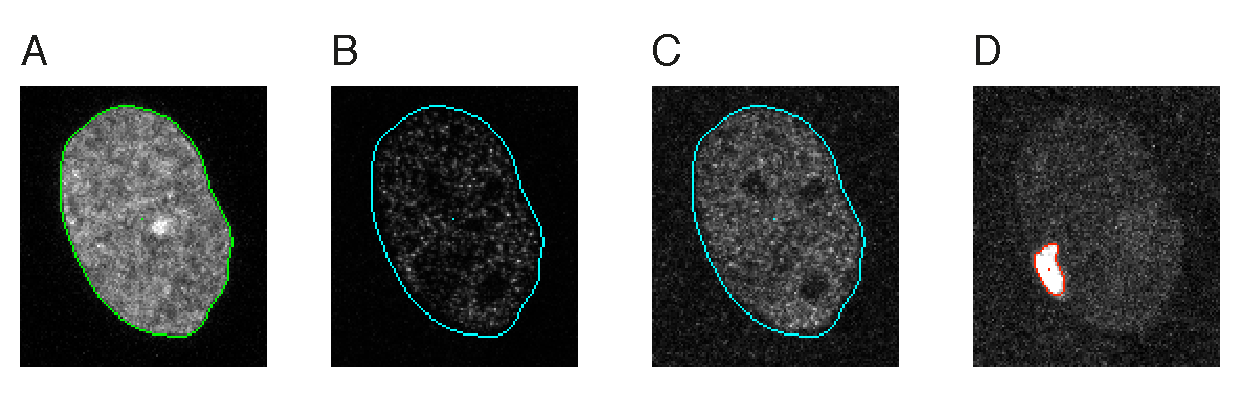
\includegraphics[width=1\textwidth]{Abbildungen/figure4_1.pdf}
		\caption{\textbf{Blubb.} A) B) }
		\label{fig:coStaining}
	\end{center}
\end{figure}

\subsection{Nuclear expression of NER factors is strongly correlated}

\begin{figure}[htbp]
	\begin{center}
		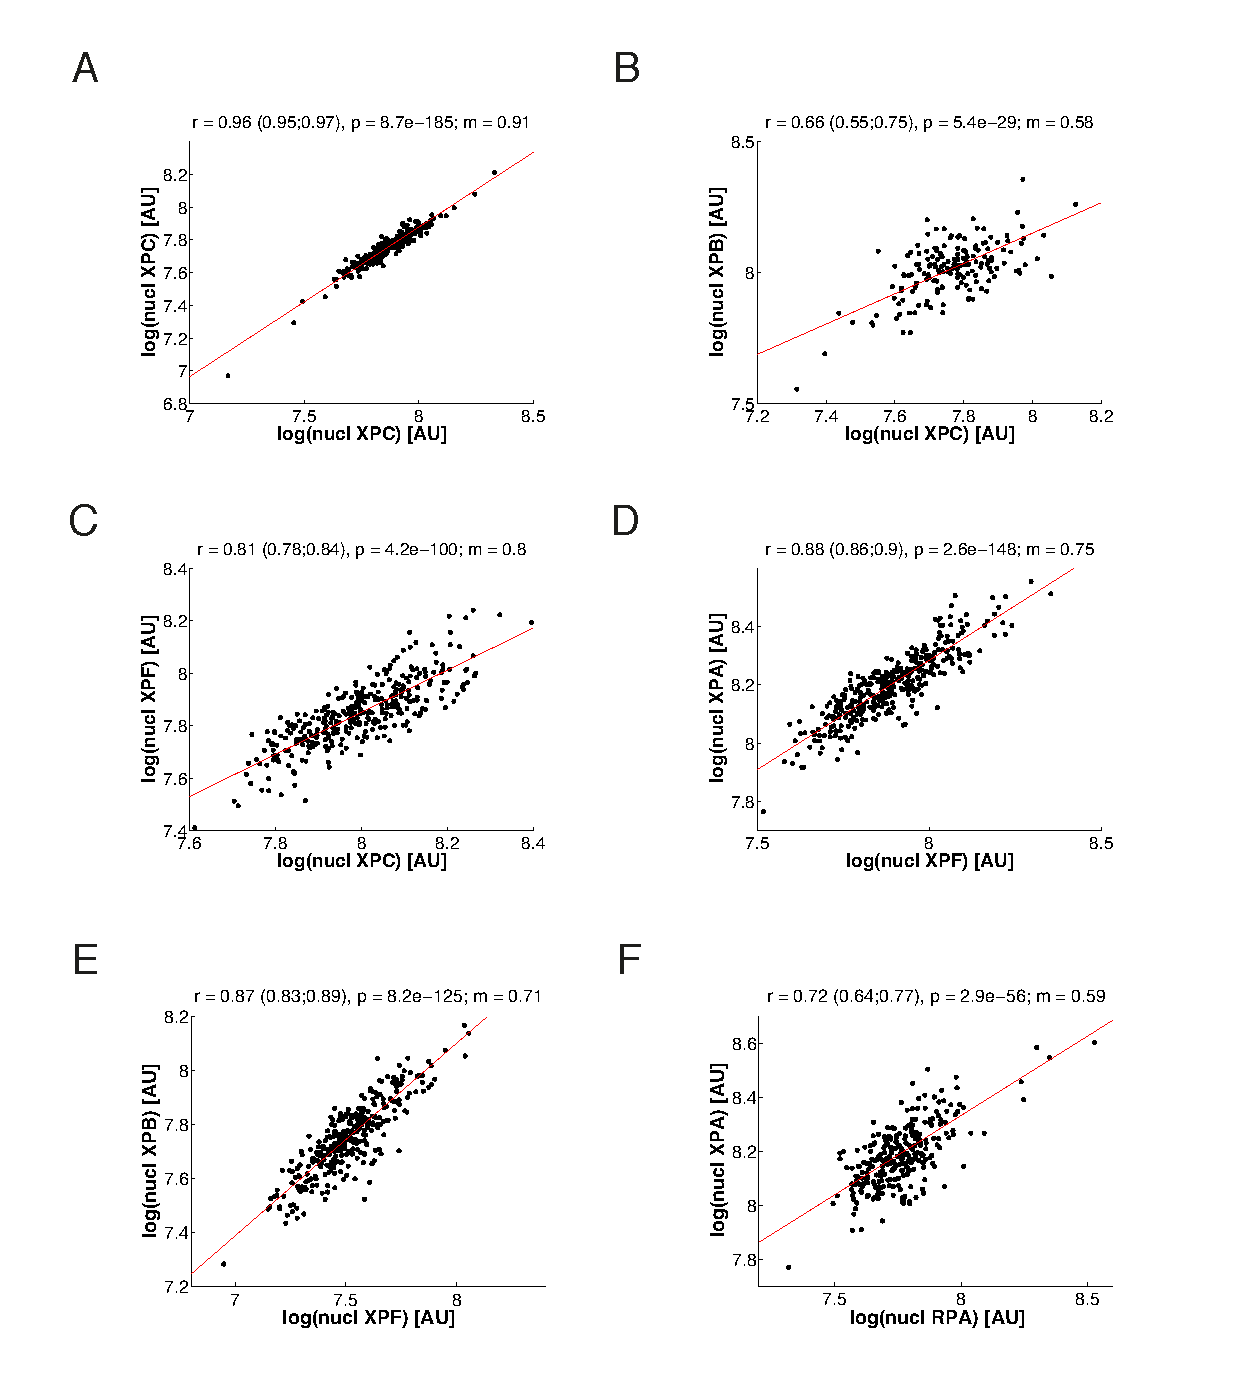
\includegraphics[width=1\textwidth]{Abbildungen/figure4_2.pdf}
		\caption{\textbf{Blubb.} A) B) }
		\label{fig:coExpressionData}
	\end{center}
\end{figure}


\begin{figure}[htbp]
	\begin{center}
		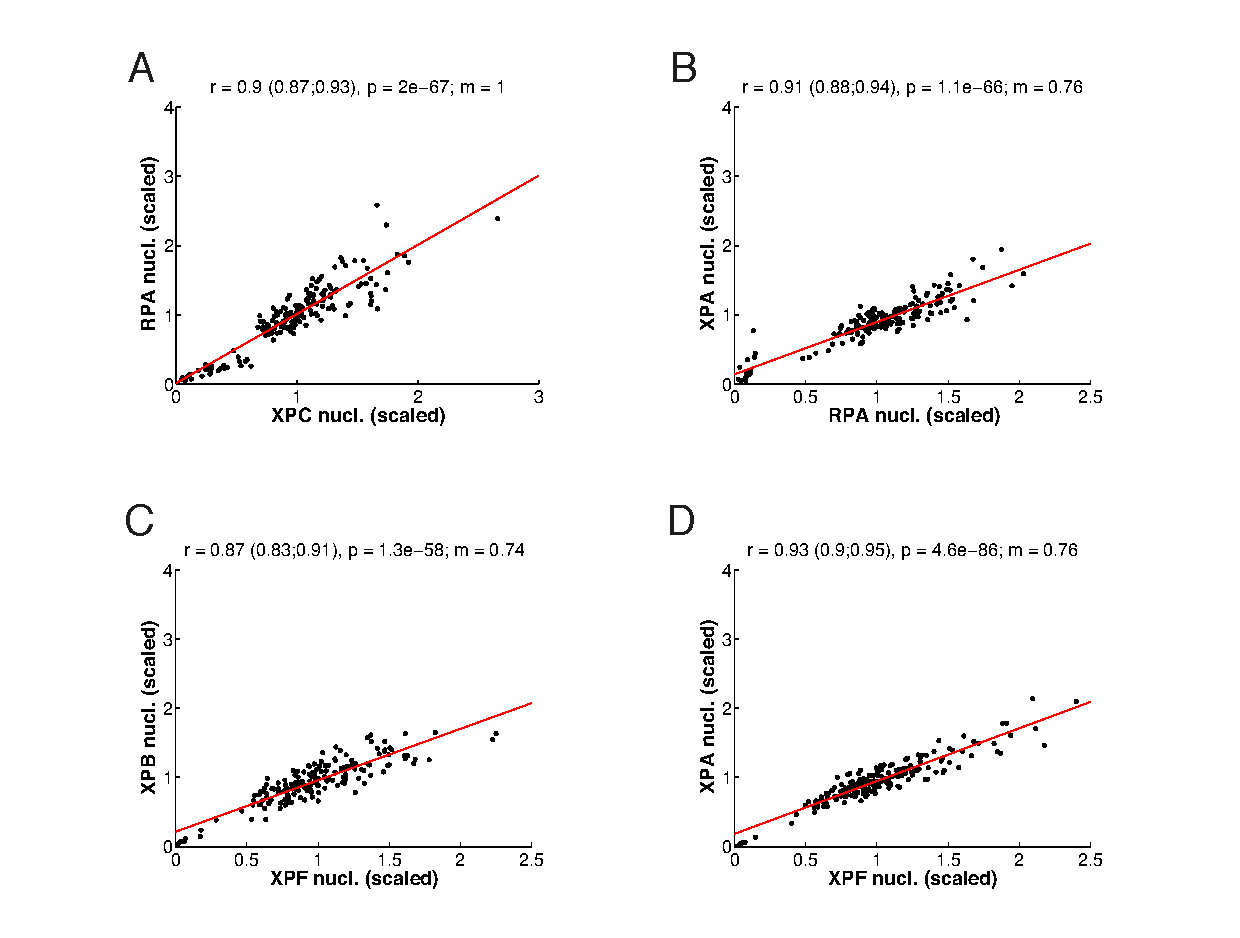
\includegraphics[width=1\textwidth]{Abbildungen/figure4_3.pdf}
		\caption{\textbf{Blubb.} A) B) }
		\label{fig:coExpressionData_woDamage}
	\end{center}
\end{figure}

\subsection{Flow cytometry verification}

\section{Consequences for the modeling}

\begin{figure}[htbp]
	\begin{center}
		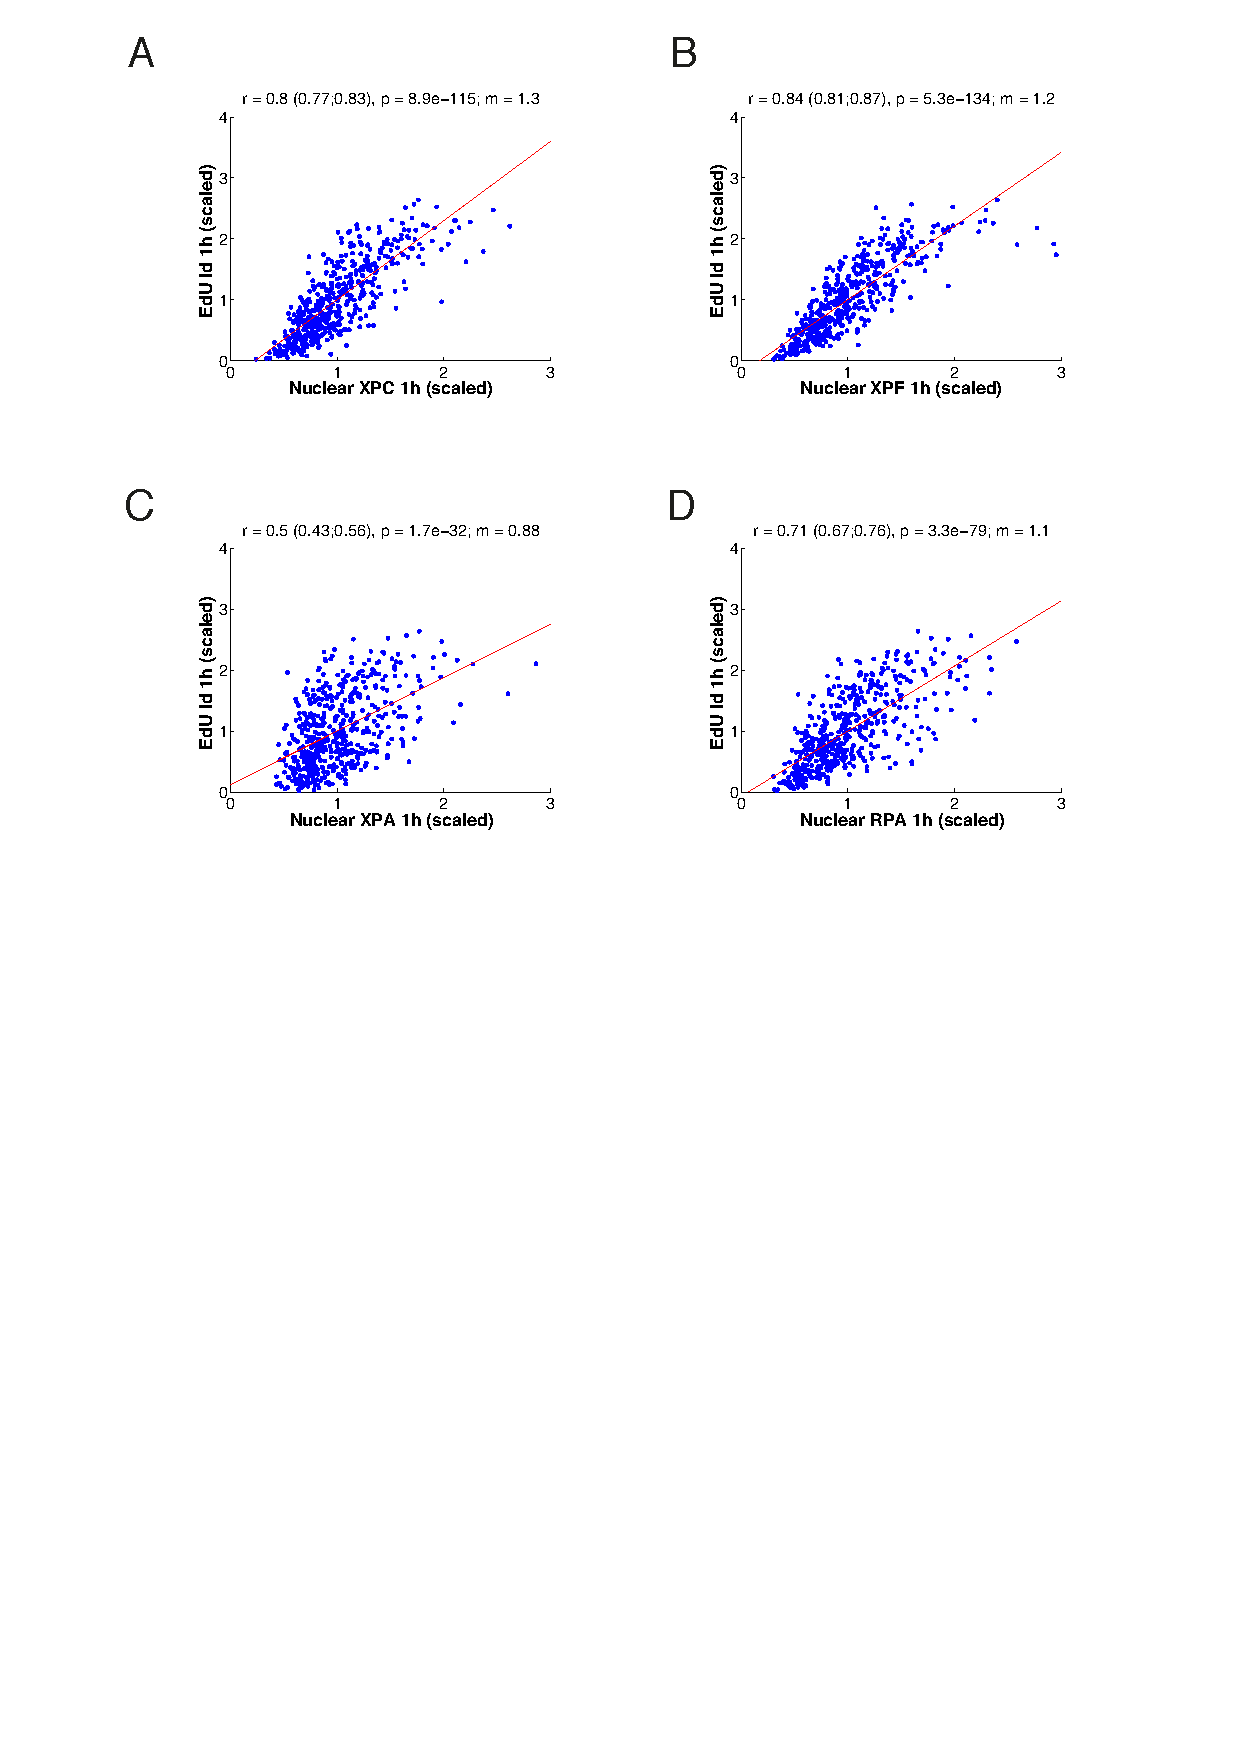
\includegraphics[width=1\textwidth]{Abbildungen/figure4_6.pdf}
		\caption{\textbf{Blubb.} A) B) }
		\label{fig:coExpressionSim}
	\end{center}
\end{figure}